\chapter{Les lignes de transmission}

\section{Résultat numérique}
\begin{wrapfigure}[13]{l}{4.5cm}
	\vspace{-5mm}
	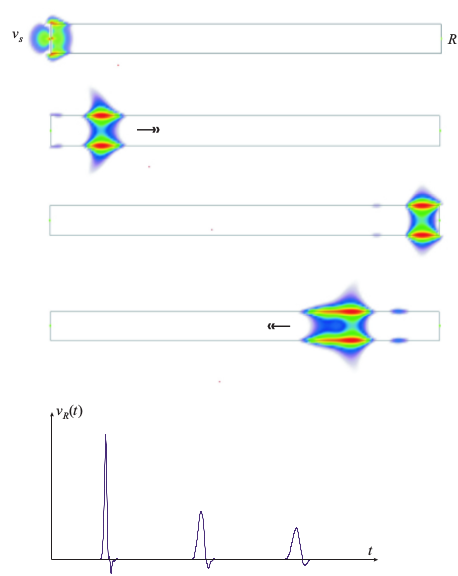
\includegraphics[scale=0.25]{ch2/image1.png}
	\captionof{figure}{ }
\end{wrapfigure}
Considérons un circuit composé uniquement d'une source de tension $s$ et d'une résistance $R$. Dans 
l'approximation quasi-statique
\begin{equation}
v_R(t) = v_s(t)
\end{equation}
Sortons de cette approximation et considérons que la tension de la source est gaussienne. Ci-dessous, 
coloré, la norme de la composante verticale du champ électrique. La ou il est non-nul, une ddp 
se crée : une \textit{onde de tension} se propage. Après $R$, une partie est \textit{réfléchie} vers 
la source. Elle peut ainsi faire plusieurs aller-retours. La \textbf{ligne de transmission} relie 
la source à la charge. Ce vocable est utilisé lorsque l'approximation quasi-statique ne s'applique 
plus. Trois types de lignes différentes sont représentées ci-dessous.
\begin{center}
	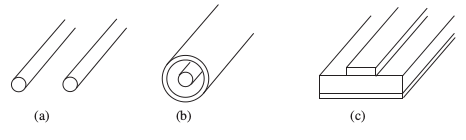
\includegraphics[scale=0.45]{ch2/image2.png}
	\captionof{figure}{(a) Ligne bifilaire (b) ligne coaxiale (c) ligne micro-ruban (microstrip). 
	Notons que l'on désigne le \textit{plan de masse} la ligne du dessous.}
\end{center}

\section{Propagation sur une ligne infinie}
La ligne infinie permet de se débarrasser des "aller-retours". Considérons une source "continue" 
de type créneau. La nouveauté est que l'on considère ici les fils : nous avons vu que la ddp entre 
ceux-ci dépend de la position et du temps : $v=v(z,t)$.\\
Considérons une source idéale $v_s$. Avant enclenchement, la ligne est neutre. Une fois celle-ci 
allumée, sous l'effet d'un champ électrique, il apparaît des densités de charges induites 
créant une ddp $v_s$. Ces charges induites provoquent l'apparition d'un champ électrique un peu 
plus loin sur la ligne : ce dernier se propage sans être atténué. Le signal n'est donc pas donné 
par le mouvement des $e^-$ (qui eux sont "plaqués" à l'extérieur de la ligne) mais par le déplacement 
du champ électrique. La ligne sert ainsi de \textit{guide} pour le champ électrique par apparition 
de charges induites.\newpage


\begin{wrapfigure}[14]{l}{5.5cm}
%	\vspace{-5mm}
	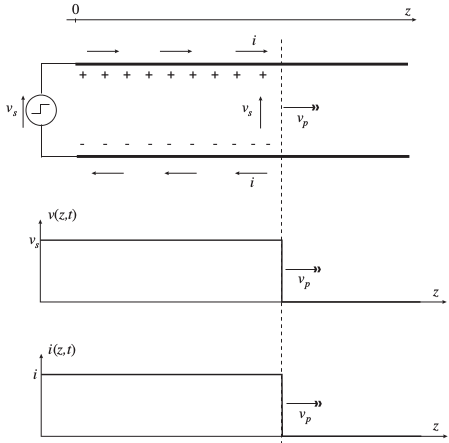
\includegraphics[scale=0.35]{ch2/image3.png}
	\captionof{figure}{ }
\end{wrapfigure}
Cette ddp $v(z,t)$ est liée à la densité de charge induite $q_l(z,t)$ par la capacité linéique de 
la ligne $C_1$
\begin{equation}
v(z,t) = \dfrac{q_l(z,t)}{C_1}
\label{eq:LienCapa}
\end{equation}
En tenant compte du délai de propagation
\begin{equation}
v(z,t) = v_s(t-z/v_p)
\end{equation}
où $v_s$ est la vitesse de propagation (inconnue). On en tire
\begin{equation}
\dfrac{\partial v}{\partial z} = -\dfrac{1}{v_p}\dfrac{\partial v}{\partial t}
\label{eq:ASat}
\end{equation}
La densité de charge induite est nulle lorsque 
le font d'onde n'est pas passé et vaut $v_sC_1$ la ou il est déjà passé : la ligne se charge. La 
ou le front d'onde est passé, les $e^-$ ont subi un déplacement microscopique formant un champ qui 
lui même, crée un courant : \textit{onde de courant}. Celle-ci doit satisfaire
\begin{equation}
\dfrac{\partial i}{\partial z} = -\dfrac{1}{v_p}\dfrac{\partial i}{\partial t}
\end{equation}
Avec cette relation et la conservation de la charge $\displaystyle\dfrac{\partial i}{\partial z} 
=-\dfrac{\partial q_l}{\partial t}$ on obtient après intégration (charge initiale et courant 
initial nuls $\forall z$)
\begin{equation}
i(z,t) = v_pq_l(z,t)
\end{equation}
En utilisant cette relation de \autoref{eq:LienCapa} on remarque que le rapport tension/courant 
est constant en tout point de la ligne\footnote{Pour une onde de tension/courant donnée.}
\begin{equation}
\dfrac{v(z,t)}{i(z,t)} = \dfrac{1}{v_pC_1}\triangleq Z_C
\label{eq:DefZC}
\end{equation}
où $Z_C$ est l'\textbf{impédance caractéristique} de la ligne : vraie pour la source en $z=0$ et 
équivalente pour la ligne infinie à une résistance de cette valeur : la ligne absorbe en 
permanence un courant $v_s/Z_c$.


\section{Les équations des lignes}
\begin{wrapfigure}[6]{r}{7.5cm}
	\vspace{-5mm}
	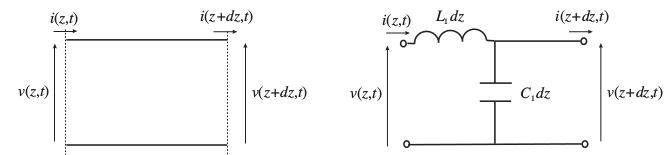
\includegraphics[scale=0.35]{ch2/image4.png}
	\captionof{figure}{ }
\end{wrapfigure}
Il faut procéder à une décomposition infinitésimale car pas d'effet de retard. Considérons 
un tel tronçon. On peut voir un tel tronçon comme une capacité valant $C_1dz$. Comme un courant 
génère un $\vec{B}$, le tronçon captera un flux : apparition d'une inductance par unité de 
longueur
\begin{equation}
L_1 = \dfrac{\phi_1}{i}
\end{equation}
Comme le tronçon est infinitésimal, la théorie des circuit s'applique. Le circuit équivalent 
peut s'écrire mathématiquement
\begin{equation}
\begin{array}{ll}
v(z+dz,t) &= v(z,t) - L_1dz\dfrac{\partial i(z,t)}{\partial t}\\
i(z+dz,t) &= i(z,t) - C_1dz\dfrac{\partial v(z,t)}{\partial t}
\end{array}
\end{equation}
où encore\\

\retenir{\ \textbf{équations des télégraphistes}.
\begin{equation}
\begin{array}{ll}
\dfrac{\partial v(z,t)}{\partial z} &= -L_1 \dfrac{\partial i(z,t)}{\partial t}\\
\dfrac{\partial i(z,t)}{\partial z} &= -C_1 \dfrac{\partial v(z,t)}{\partial t}
\end{array}
\label{eq:Telegraphistes}
\end{equation}}\ 

Ces équations montre que le courant correspond au courant injecté, diminué du courant de 
fuite dans les capacités. En découplant le système (remplace l'une dans l'autre après 
en avoir dérivée une) en augmentant l'ordre, on retrouve les équations d'ondes
\begin{equation}
\begin{array}{ll}
\dfrac{\partial^2 v(z,t)}{\partial z^2} &= L_1C_1\dfrac{\partial^2 v(z,t)}{\partial t^2}\\
\dfrac{\partial^2 i(z,t)}{\partial z^2} &= L_1C_1\dfrac{\partial^2 i(z,t)}{\partial t^2}
\end{array}
\end{equation}
Les tensions et courants se propagent donc à la vitesse 
\begin{equation}
v_p = \dfrac{1}{\sqrt{L_1C_1}}
\end{equation}
On peut écrire, à partir de la définition \autoref{eq:DefZC} de $Z_C$\\
\retenir{\begin{equation}
Z_C = \sqrt{\dfrac{L_1}{C_1}}
\end{equation}}\ \\

\begin{wrapfigure}[9]{r}{4cm}
	\vspace{-5mm}
	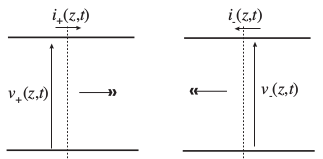
\includegraphics[scale=0.35]{ch2/image5.png}
	\captionof{figure}{Onde progressive (gauche) et régressive (droite)}
\end{wrapfigure}
La solution de ces équations est bien connues : il s'agit d'ondes progressives (droite) ou 
régressives (gauche) se déplaçant à vitesse constante. Le premier type de solution à la 
forme
\begin{equation}
v_+(z,t) = V_+f(t-z/v_p)\qquad V_+\in\mathbb{R}
\end{equation}
où $f$ est une fonction quelconque. Cette solution satisfaisant \autoref{eq:ASat} correspond 
à une tension se propageant le long de la ligne sans atténuation ni déformation. Pour trouver 
le courant $i_+(z,t)$ associé, on utilise
\begin{equation}
\left\{\begin{array}{l}
\autoref{eq:ASat}\\
\autoref{eq:Telegraphistes}
\end{array}\right.\quad\Longrightarrow\quad \dfrac{\partial i_+(z,t)}{\partial t} = 
\dfrac{1}{v_pL_1}\dfrac{\partial v_+(z,t)}{\partial t}
\end{equation}
Après intégration (C.I. nulles)
\begin{equation}
i_+(z,t) = \dfrac{v_+(z,t)}{Z_c}
\end{equation}
Le second type de solution (régressive) est de la forme
\begin{equation}
v_+(z,t) = V_-g(t+z/v_p)\qquad V_-\in\mathbb{R}
\end{equation}
On peut déduire le courant $i_-(z,t)$ (conventionnellement choisi opposé à $i(z,t)$, 
le courant étant défini positif de gauche à droite sur la ligne supérieur) associé à 
cette onde par résolution de l'ED suivante (similairement au cas de l'onde progressive)
\begin{equation}
\dfrac{\partial i_(z,t)}{\partial t} = -
\dfrac{\partial i(z,t)}{\partial t} = \dfrac{1}{v_pL_1}\dfrac{\partial v_-(z,t)}{\partial t}
\end{equation}
Après intégration
\begin{equation}
i_-(z,t) = \dfrac{v_-(z,t)}{Z_c}
\end{equation}
En fonction de l'écho, nous aurons l'une ou l'autre solution. La tension en un point est 
obtenue en sommant toutes les tensions de toutes les ondes progressives et régressive. Par 
contre, pour le courant, il faut effectuer la différence par convention. A cause de cette 
différence, la tension divisée par le courant ne vaut pas $Z_C$ globalement (mais bien en 
un point)


\section{Réflexions}
	\subsection{Coefficients de réflexion}
	Soit une ligne de transmission sans pertes, uniforme, guidant une onde progressive, 
	de longueur finie $L$. Si $R=R_C$, la condition sur la tension et le courant à ses 
	bornes s'écrit
	\begin{equation}
	\dfrac{v(L,t)}{i(L,t)} = Z_c
	\end{equation}
	Soit la relation précédemment trouvée : l'onde n'est pas perturbée par la présence de 
	la résistance et pas de formation d'onde réfléchie (entièrement absorbé par la 
	résistance\footnote{"Les charges induites associées à l'onde, "s'écoulent" dans la 
	résistance pour y former un courant"}) : la résistance de charge est \textbf{adaptée}, 
	c'est le cas optimal (rien n'est renvoyé à la source. Si $R\neq Z_c$ 
	\begin{equation}
	\dfrac{v(L,t)}{i(L,t)} = R
	\label{eq:PlusZcMaisR}
	\end{equation}
	Ce qui n'est plus compatible avec \autoref{eq:DefZC} : la quantité de charges induites 
	associée à l'onde ne correspond plus à la valeur du courant exigée par $R$ : perturbation 
	de l'onde et apparition d'une onde réfléchie :
	\begin{equation}
	\begin{array}{ll}
	v(L,t) &= v_+(L,t) + v_-(L,t)\\
	i(L,t) &= i_+(L,t) - i_-(L,t)	= \dfrac{v_+(L,t)}{Z_c}-\dfrac{v_-(L,t)}{Z_c}
	\end{array}
	\end{equation}
	On définit alors $\Gamma_L$, la fraction de l'onde incidente réfléchie : le 
	\textbf{coefficient de réflexion} à la charge
	\begin{equation}
	\Gamma_L = \dfrac{v_-(L,t)}{v_+(L,t)} = \dfrac{i_-(L,t)}{i_+(L,t)}
	\end{equation}
	Avec \autoref{eq:PlusZcMaisR} on trouve\\
	\retenir{\begin{equation}
	\Gamma_L = \dfrac{R-Z_c}{R+Z_c}
	\end{equation}}
	Lorsque la ligne est court-court-court-circuitée $R=0 \rightarrow \Gamma_L=-1$ : tension nulle en 
	bout de ligne. Lors que la ligne est ouverte $R=\infty \rightarrow \Gamma = 1$ (courant 
	nul en fin de ligne). L'onde revient à la source et le même phénomène se produit (remplacer 
	$R$ par $R_S$) : nouvelle onde progressive qui se propage !
	
	\subsection{Application}
	Voir page 21-23 : rien de compliqué, ce ne sont que des math. Quelque commentaires sur 
	l'équation (2.30) du syllabus. Le premier terme correspond à un aller, le second au 
	retour, le troisième à un aller-retour, \dots En mettant $\Gamma_L$ en évidence, on fait 
	apparaître une série géométrique. Ces calculs décrivent ainsi un état transitoire : après 
	allumage de la source, on observe plusieurs échos jusqu'à une stabilisation vers le 
	résultat quasi-statique.
	
\section{Les lignes en régime sinusoïdal permanent}
	\subsection{Tension et courant sur la ligne}
	Considérons cette fois-ci une source sinusoïdale : légèrement plus compliqué, car tout 
	variera de façon sinusoïdale également (en supposant que la charge en fin de ligne est 
	linéaire).
	\begin{equation}
	v_s(t) = V_S\ \cos(\omega t + \phi_s) = \Re\left(\underline{V_S}e^{j\omega t}\right)
	\end{equation}
	où $V_s$ est l’amplitude de la tension, $\phi_s$ sa phase, $\omega$ sa pulsation et 
	$\underline{V_S} = V_Se^{j\phi_s}$, un phaseur.\\
	On peut faire de même pour les tensions et courants
	\begin{equation}
	\begin{array}{ll}
	v(z,t) &= \Re \left(\underline{V}(z)e^{j\omega t}\right)\\
	i(z,t) &= \Re \left(\underline{I}(z)e^{j\omega t}\right)	
	\end{array}
	\end{equation}
	\danger Ces phaseurs dépendent ici de $z$ ! On peut ré-écrire les équations des 
	télégraphistes\\
	\retenir{\begin{equation}
	\begin{array}{ll}
	\dfrac{d\underline{V}(z)}{dz} &= -j\omega L_1 \underline{I}(z)\\
	\dfrac{d\underline{I}(z)}{dz} &= -j\omega C_1 \underline{V}(z)	
	\end{array}
	\end{equation}}\ \\
	
	On peut, comme précédemment, découpler le système
	\begin{equation}
	\begin{array}{lll}
	\dfrac{d^2\underline{V}(z)}{dz^2} &= -\omega^2 L_1C_1\underline{V}(z) &= -\beta^2
	\underline{V}(z)\\
	\dfrac{d^2\underline{I}(z)}{dz^2} &= -\omega^2 L_1C_1\underline{I}(z) &= -\beta^2
	\underline{I}(z)	
	\end{array}
	\end{equation}
	où $\beta = \omega\sqrt{L_1C_1}$. La résolution de ces équations donne
	\begin{equation}
	\begin{array}{lll}
	\underline{V_+}(z) = V_+e^{-j\beta z},\qquad\qquad 	\underline{V_-}(z) &= V_-e^{j\beta z}\\
	\underline{I_+}(z) = I_+e^{-j\beta z},\qquad\qquad 	\underline{I_-}(z) &= I_-e^{j\beta z}	
	\end{array}
	\end{equation}
	Nous avons travailler en phaseur : il s'agit de la situation en régime décrite par la 
	superposition d'une seule onde progressive et une seule onde régressive.
	\begin{equation}
	\begin{array}{ll}
	\underline{V}(z) &= V_+e^{-j\beta z}+V_-e^{j\beta z}\\
	\underline{I}(z) &= I_+e^{-j\beta z}-I_-e^{j\beta z}	
	\end{array}
	\end{equation}
	En utilisant les équations des télégraphistes, on obtient
	\begin{equation}
	\dfrac{V_+}{I_+} = \dfrac{V_-}{I_-} = Z_c
	\end{equation}
	Notons que le terme d'exponentielle imaginaire correspond aux changement de phases dus 
	au délai de propagation. Pour voir une phase constante (argument constant), il faut se 
	déplacer à vitesse
	\begin{equation}
	\dfrac{\omega}{\beta} = \dfrac{1}{\sqrt{L_1C_1}} = v_p
	\end{equation}
	soit la \textbf{vitesse de phase} (qui vaut bien la vitesse de propagation sur la ligne).
	La longueur d'onde, elle, vaut $\lambda = \dfrac{2\pi}{\beta}$.
	
	\newpage
	\subsection{Application}
	Avec $Z_C$, on peut écrire la tension et le courant le long de la ligne
	\begin{equation}
	\begin{array}{ll}
	\underline{V}(z) &= V_+e^{-j\beta z} + V_-e^{j\beta z}\\
	\underline{I}(z) &= \dfrac{V_+}{Z_c} e^{-j\beta z} - \dfrac{V_-}{Z_c}e^{j\beta z}	
	\end{array}
	\label{eq:2.45}
	\end{equation}
	En $Z=L$
	\begin{equation}
	\dfrac{\underline{V}(L)}{\underline{I}(L)} = Z_L
	\end{equation}
	En définissant le coefficient de réflexion à la charge
	\begin{equation}
	\Gamma_L = \dfrac{\underline{V}_-(L)}{\underline{V}_+(L)} = \dfrac{V_-}{V_+}e^{2j\beta L}
	\label{eq:2.47}
	\end{equation}
	On peut alors écrire la condition en bout de ligne
	\begin{equation}
	Z_L = Z_c\dfrac{1+\Gamma_L}{1-\Gamma_L}\quad\Leftrightarrow\quad \Gamma_L = \dfrac{Z_l-Z_c}{
	Z_l+Z_c}
	\end{equation}
	Les C.I permettent de déterminer $V_+$ et $V_-$. Le calcul ne sera pas détaillé ici. Discutons 
	néanmoins l'expression obtenue
	\begin{equation}
	V_+ = \dfrac{Z_c}{Z_S+Z_c}\left(1+\Gamma_L\Gamma_Se^{-2j\beta L}+\Gamma_L^2\Gamma_S^2e^{-4j\beta L}
	+\dots\right)\underline{V_S}
	\end{equation}
	\begin{wrapfigure}[11]{r}{6.5cm}
	\vspace{-5mm}
	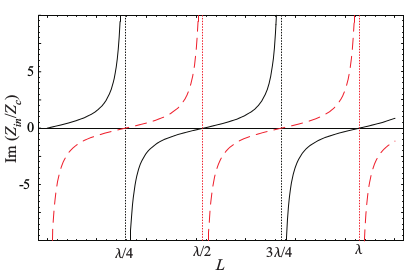
\includegraphics[scale=0.45]{ch2/image6.png}
	\captionof{figure}{ }
	\end{wrapfigure}
	La tension en situation de régime est la superposition de la tension appliquée par la source et de 
	l'ensemble des échos (chaque exp. correspond au délai supplémentaire de chaque écho). Cette 
	expression est intéressante car celle-ci dépend de $L$. Plaçons-nous en $L=\lambda/4$ : la ligne 
	se comporte comme un circuit ouvert. En augmentant $L$, la partie imaginaire devient négative : 
	elle se comporte comme une capacité. On repasse ensuite par $Z=0$, puis on retrouve un comportement 
	inductif. Il s'agit de la courbe pleine ci-contre.\\
	Analysons maintenant la courbe en pointillée correspondant à une ligne \textit{ouverte} (!). Si 
	$L=\lambda/4$, le générateur "verra" un circuit fermé ! On voit dès lors qu'à partir d'une ligne, 
	il est possible de réaliser ce que l'on souhaite rien qu'en jouant sur la longueur.
	
	\subsection{Impédance d'entrée}
	L'impédance d'entrée de la ligne est celle vue par la source 
	\begin{equation}
	Z_{in} = \dfrac{\underline{V}(0)}{\underline{I}(0)}
	\end{equation}
	Avec \autoref{eq:2.45} et \autoref{eq:2.47} :
	\begin{equation}
	\begin{array}{ll}
	\underline{V}(z) &= V_+\left(e^{-j\beta z} + \Gamma_L e^{-2j\beta L}e^{j\beta z}\right)\\
	\underline{V}(z) &= \dfrac{V_+}{Z_c} \left(e^{-j\beta z} + \Gamma_L e^{-2j\beta L}e^{j\beta z}\right)	
	\end{array}
	\end{equation}
	Par définition de $Z_{in}$\\
	\retenir{\begin{equation}
	Z_{in} = Z_c\dfrac{1+\Gamma_L e^{-2j\beta L}}{1-\Gamma_Le^{-2j\beta L}}
	\end{equation}}\ \\
	
	L'impédance d'entrée va non seulement dépendre de l'impédance de charge connectée, mais également de 
	la longueur de la ligne.
	
	
	
	
	
	
	
	
	
	
	
	
	
	
	
	
	
	
	
	
	
	
	
	
	
	
	
	
	
	
	
	
	
	
	
	
	
	
	



